% -*- coding: utf-8 -*-
\chapter{Entropies in Solvation}\label{entropies}

In this section, we present an already published paper in which we
adress the entropies in solvation.

Les entropies représentent une contribution fondamentale à l'énergie libre de
Gibbs, porteuse d'informations chimiques essentielles, notamment dans l'étude
des mécanismes réactionnels. Toutefois, leur évaluation en solution reste une
tâche loin d'être triviale. Dans ce travail, nous nous concentrons sur cette
évaluation dans le cadre des modèles de solvatation implicites. Pour cela, des
corrections successives ---de complexité croissante--- sont proposées. Elles ne
font appel qu'à des grandeurs accessibles via tout programme standard de chimie
quantique ainsi qu'à des propriétés macroscopiques du solvant. Ces modèles sont
évalués par comparaison à plus d'une centaine de valeurs expérimentales
d'entropie mesurées en phase liquide. Il en ressort qu'une amélioration
significative par rapport à l'approximation classique du gaz perfect peut être
obtenue à un coût computationnel quasi négligeable, menant à un modèle
prédictif à la fois robuste et transférable.

\newpage
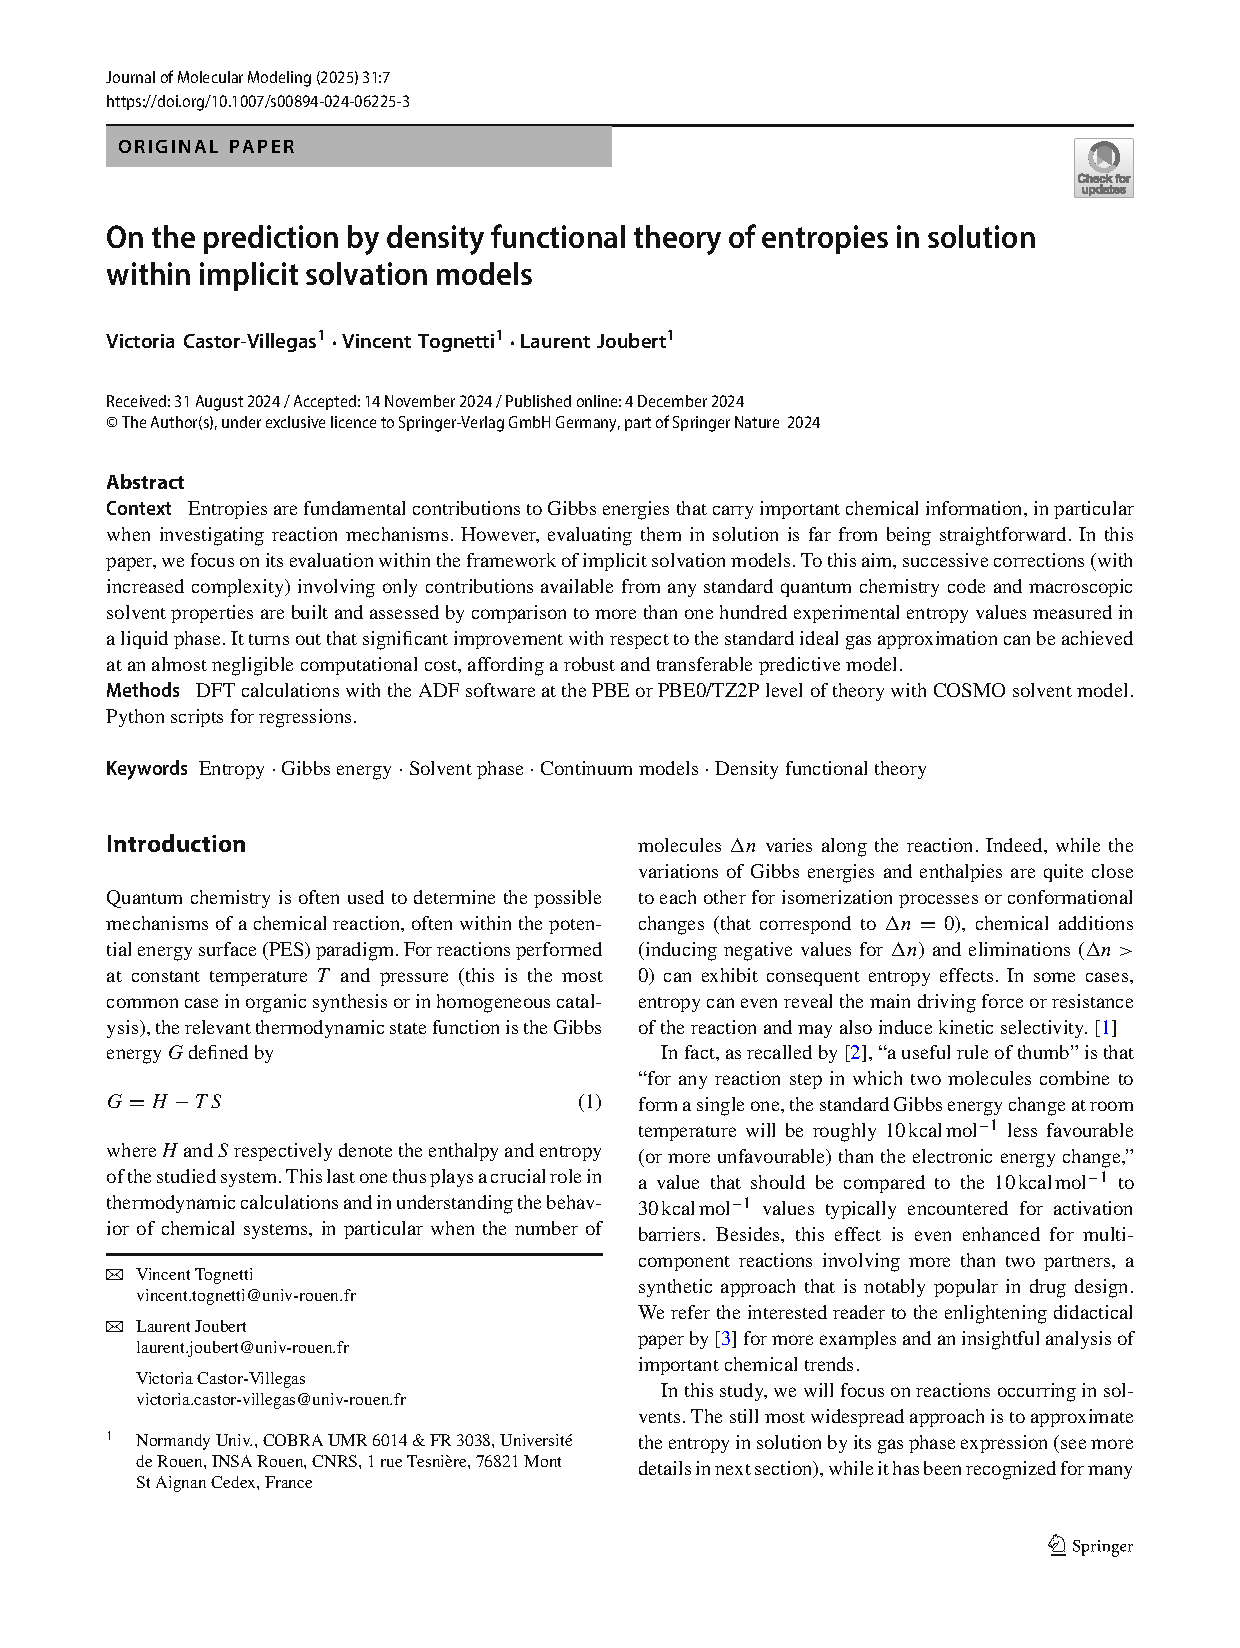
\includepdf[pages=-]{paper_entropies.pdf}

